\section{Accumulated Muon Deflection}\label{sec:accum_defl}

As shown in Section~\ref{sec:defl_per_int}, in general the deflection per interaction 
is lower $\sim\SI{1}{\degree}$. Since these deflections accumulate along the 
propagation path, the angle between the incoming muon direction and the outgoing 
muon direction is analyzed. The deflection results as a limit on the 
angular reconstruction accuracy.

At first, the deflections in PROPOSAL are compared to 
the tools MUSIC \cite{MUSIC,comparison_MUSIC_GEANT4_2009} and GEANT4 \cite{GEANT4}.
MUSIC (MUon SImulation Code) is a tool to simulate the propagation of muons 
through media like rock and water considering the same energy losses as in 
PROPOSAL. Also, the losses are divided into continuous and stochastic 
energy losses by a relative energy cut. Several cross-sections, multiple scattering 
methods and parametrizations for stochastic deflection are 
available. For these studies, it is chosen bremsstrahlung \cite{Bremsstrahlung_KKP}, 
nuclear interaction \cite{nulcint_bugaev_Shlepin, bugaev_1980_defl,bugaev_1981_defl} 
and electron pair production \cite{epair_kelner,epair_kokoulin_petrukhin}, 
which deflections are parametrized by \cite{Van_Ginneken}. 
Also, ionization is treated as a stochastic process with the Bethe-Bloch 
formula including knock-on electron production. As scattering, the gaussian 
approximation \cite{HIGHLAND_1975} is set. 
GEANT4 is another common toolkit to simulate the passage of particles through 
a medium with several possibilities and a focus on high-energy 
particle accelerators \cite{GEANT4}. 

A comparison of all three tools is done in Figure~\ref{fig:compare_MUSIC} 
with four different settings in PROPOSAL for the 
accumulated deflection angle $\theta_{\text{acc}}$ and the lateral displacement
$x$. The deflection angles are very similar in all cases. The 
displacement is dominated by GEANT4 and PROPOSAL with Molière scattering, which 
leads to the largest deflections and thus to a larger displacement. 
PROPOSAL with Highland scattering and MUSIC have less outliers, since large 
deflections are neglected in the Gaussian approximation \cite{HIGHLAND_1975}. 
The combination of Highland and \cite{Van_Ginneken} leads to the smallest 
displacement, since in nuclear interaction, the sampling from the root mean squared angle in the 
exponential distribution neglects outliers to larger angles.

Detailed information are given in Table~\ref{tab:compare_MUSIC}. In GEANT4, the 
largest deflections result with $\overline{\theta} = \SI{0.27}{\degree}$ 
and $\overline{x} = \SI{3.3}{\meter}$. The lowest values $\overline{\theta} = \SI{0.22}{\degree}$ and 
$\overline{x} = \SI{2.6}{\meter}$ result in MUSIC. The results of PROPOSAL lay between 
these two tools for all four settings which approves the 
correctness of PROPOSAL.

A measurement of muon deflection in low-Z materials was done in \cite{attwood_2006}. 
From this it can be seen that for $Z < 4$ the scattering angle is overestimated 
by Molière scattering in GEANT4. Hence, the lower scattering in PROPOSAL leads 
to a better precision especially in the region of outliers. The simulation is 
done in liquid $\text{H}_2$ with a thickness of $\SI{109}{\milli\meter}$ and an 
initial particle energy of $E_{\mathrm{i}} = \SI{199}{\mega\electronvolt}$. 
The result is presented in Figure~\ref{fig:attwood_comparison}.
\begin{figure}
    \centering 
    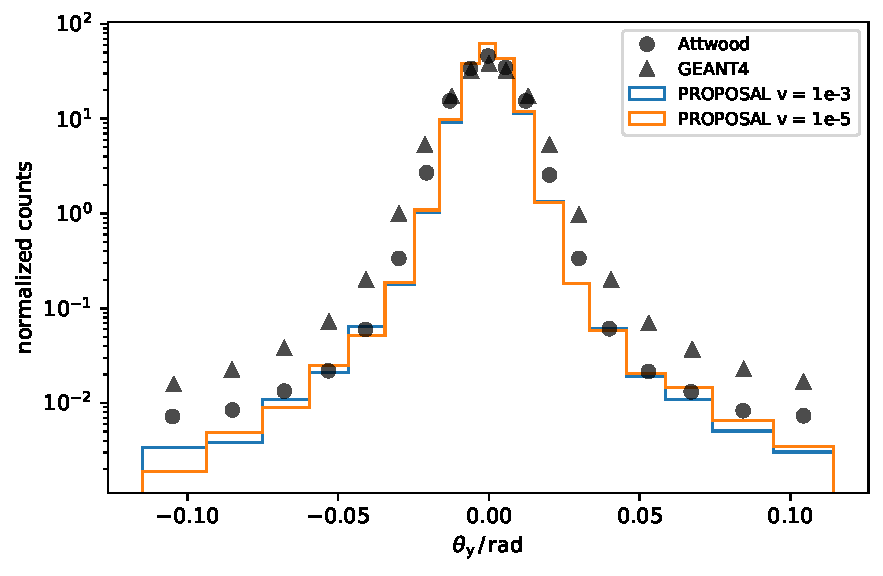
\includegraphics[width=0.8\textwidth]{../../deflection/plots/FINAL/attwood_comparison_moliere_E199MeV_final.pdf}
    \caption{In total $\num{e5}$ muons with $E_{\mathrm{i}} = \SI{199}{\mega\electronvolt}$ are propagated through 
    $\SI{109}{\milli\meter}$ of liquid $\text{H}_2$. In PROPOSAL, the simulation is done 
    for two different energy cuts $\texttt{v\_cut} = \num{e-3}$ and $\texttt{v\_cut} = \num{e-5}$ using Molière scattering.
    Measured data of Attwood and simulation data of GEANT4 are taken from \cite{attwood_2006}. The figure presents 
    the normalized counts in dependence of the projected scattering angle $\theta_{\mathrm{y}}$ in radians. At small deflections, PROPOSAL 
    is underestimating, but at larger deflections the result seems to be more accurate than GEANT4's.}
    \label{fig:attwood_comparison}
\end{figure}

% \begin{itemize}
%     \item this is MUSIC: 
%     \item electron pair production:  Kelner-..[\cite{epair_kelner,epair_kokoulin_petrukhin}], deflection [\cite{Van_Ginneken}]
%     \item bremsstrahlung: Kelner, Kokoulin andPetrukhin
%     [\cite{Bremsstrahlung_KKP}], deflection [\cite{Van_Ginneken}] 
%     \item inelastic scattering: shlepin and Bugaev [\cite{nulcint_bugaev_Shlepin}], \cite{bugaev_1980_defl,bugaev_1981_defl} (überprüfe, ob genau diese referenz auch im GEANT4 verwendet wird!!!)
%     \item ionization: treated as stochastic process (Bethe-Bloch formula) including knock-on electron production, but no deflection
%     \item scattering: gaussian approx \cite{HIGHLAND_1975}
% \end{itemize}

% \textcolor{red}{Moliere beschreibt nur die Winkeländerung, jedoch nicht die laterale Verschiebung. Wie machen wir das mit der 
% laterale Verschiebung in PROPOSAL für Moliere? Gaussian approx berücsichtigt die Verschiebung}

% \begin{itemize}
%     \item this is GEANT4
%     \item electron pair production: 
%     \item bremsstrahlung:
%     \item inelastic scattering: cross-section \cite{Borog:1975_inelastic}, deflection \cite{Borog:1977_inelastic,Borog:1975_inelastic}
%     \item ionization:
%     \item scattering:
% \end{itemize}

% \begin{itemize}
%     \item this is PROPOSAL
%     \item electron pair production: KelnerKokoulinPetrukhin (Proc. 12th ICCR (1971), 2436) with corrections for the interaction with atomic electrons (Phys. Atom. Nucl. 61 (1998), 448) [\cite{}], deflection \cite{Van_Ginneken}
%     \item bremsstrahlung: KelnerKokoulinPetrukhin (Preprint MEPhI (1995) no. 024-95) and (Phys. Atom. Nucl. 62 (1999), 272) [\cite{}], deflection \cite{Van_Ginneken,GEANT4}
%     \item inelastic scattering: AbramowiczLevinLevyMaor97 (arXiv::hep-ph/9712415) \cite{} with shadowing ButkevichMikheyev (JETP 95 (2002), 11) \cite{}, deflection \cite{Van_Ginneken, Borog:1977_inelastic,Borog:1975_inelastic}
%     \item ionization: BetheBlochRossi Ionization described by Bethe-Bloch formula with corrections for muons and taus by (B. B. Rossi. Prentice-Hall, Inc., Englewood Cliffs, NJ, 1952) [\cite{}], deflection [direct calculation using four-momentum transfers]
%     \item scattering: \cite{HIGHLAND_1975,moliere_scattering}
% \end{itemize}


\begin{figure}
    \centering
    \subcaptionbox{
        The accumulated deflection $\theta_{\mathrm{acc}}$ in degree is very similar in all cases.
        \label{fig:compare_MUSIC_degree}}
        {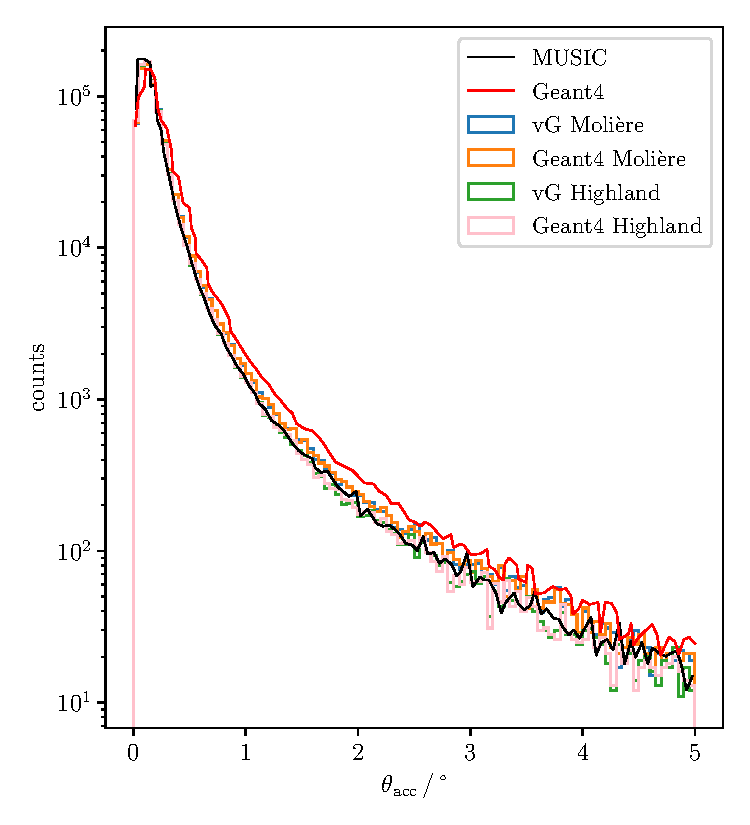
\includegraphics[width=0.48\textwidth]{../../deflection/plots/FINAL/2TeV_1e6events_accumulated_defl_only3km_5deg_paper.pdf}}
    \subcaptionbox{
        The lateral displacement $x$ in meter depends 
        on the scattering method. Molière scattering leads to larger distances.
        \label{fig:compare_MUSIC_dist}}
        {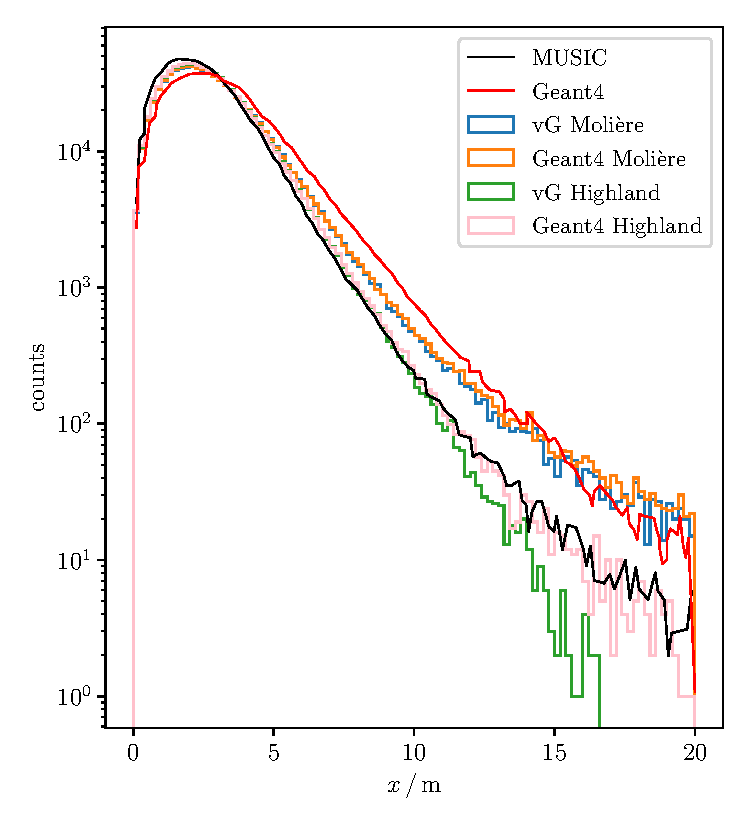
\includegraphics[width=0.48\textwidth]{../../deflection/plots/FINAL/2TeV_1e6events_distance_showeraxis_only3km_20m_paper.pdf}}
    \caption{A comparison of the results of MUSIC, GEANT4 and PROPOSAL is presented for $\num{1000000}$ negative charged muons propagated with 
    $E_{\text{i}} = \SI{2}{\tera\electronvolt}$ over a distance of 
    $\SI{3}{\kilo\meter}$ in water. A $\texttt{v\_cut} = 0.001$ is set. In PROPOSAL, 
    bremsstrahlung and photonuclear interaction are parametrized by 
    Van Ginneken (vG) and GEANT4 and both scattering methods are checked. Detailed information are given in 
    Table~\ref{tab:compare_MUSIC}. The results for MUSIC and GEANT4 are taken from 
    \cite{comparison_MUSIC_GEANT4_2009}.}
    \label{fig:compare_MUSIC}
\end{figure}



\begin{table}
    \small
    \centering
    \caption{The survival probability $p_{\text{s}}$ - otherwise the muon decays before, the mean survived muon 
    energy $\overline{E}_{\text{f}}$, the mean scattered angle $\overline{\theta}$ 
    and the mean displacement $\overline{x}$ are presented for all cases from 
    Figure~\ref{fig:compare_MUSIC}. For all means, the standard deviation is given.
    The largest deflection and displacement result in the tool GEANT4, which has the lowest mean survived energy. The lower the energy, the larger the deflection.}
    \begin{tabular}{l|cc|cccc}
        \toprule
        & & & \multicolumn{4}{c}{PROPOSAL} \\
        &  & & \multicolumn{2}{c}{Molière} & \multicolumn{2}{c}{Highland} \\
        & MUSIC & GEANT4 & vG & GEANT4 & vG & GEANT4 \\
        \midrule
        $p_{\text{s}}\,/\,\si{\percent}$ & 77.9 & 79.3 &  \multicolumn{4}{c}{77.9}\\
        $\overline{E}_{\text{f}}\,/\,\si{\giga\electronvolt}$ & 323 & 317 & \multicolumn{4}{c}{331$\pm$178} \\
        $\overline{\theta}\,/\,\si{\degree}$ & 0.22 & 0.27 & 0.24$\pm$0.45 & 0.24$\pm$0.45 & 0.22$\pm$0.35 & 0.22$\pm$0.35   \\
        $\overline{x}\,/\,\si{\meter}$ & 2.6 & 3.3 & 2.9$\pm$2.6 & 2.9$\pm$2.6 & 2.7$\pm$1.6 & 2.7$\pm$1.7  \\
     \bottomrule
    \end{tabular}
    \label{tab:compare_MUSIC}
\end{table}




For current analyses, it is important to study the impact of the muon 
deflection on the angular resolution to estimate an uncertainty on the reconstruction.
For this purpose, four different initial energies 
from $E_{\text{i}} = \SI{10}{\tera\electronvolt}$ to 
$E_{\text{i}} = \SI{10}{\peta\electronvolt}$ are used and the final 
energy is set to $E_{\text{f,\,min}} \geq \SI{10}{\giga\electronvolt}$ with 
$E_{\text{f,\,min}} < E_{\text{i}}$ for each simulation. To compare the results of 
a total of $\num{36}$ simulations, the median of the deflection distribution 
with a $\SI{95}{\percent}$ central interval is presented in 
Figure~\ref{fig:fit_median}.
The lower the final muon energy, the larger the accumulated deflection. 
For energies $E_{\text{f}} = \SI{1}{\peta\electronvolt}$, the median deflection 
is lower than $\SI{e-3}{\degree}$. For energies $E_{\text{f}} = \SI{10}{\giga\electronvolt}$, 
angles larger than $\SI{1}{\degree}$ are possible. For an energy range 
$E_{\text{f}} \approx \SI{500}{\giga\electronvolt} - \SI{1}{\tera\electronvolt}$, 
there is a small overlap of the deflection with the angular resolution of KM3NeT 
\cite{KM3NeT_Resolution2016}. The resolution of IceCube is a bit worse and 
therefore not affected \cite{IceCube_Resolution2021}. Since these simulations are done 
in ice, the same simulations are done in water. The deviations of the medians
are less than $\SI{1}{\percent}$ for all energies.

Furthermore, in Figure~\ref{fig:fit_median} there are only $12$ medians visible, 
instead of $36$ which is the total amount of all simulations. This result points 
out that the total deflection of a muon 
primarily depends on the final muon energy.
The initial muon energy is negligible. 
Hence, the reconstructed muon 
energy in a detector can be used to estimate a theoretical deflection. For this 
purpose, the following fit-function 
\begin{equation}
     f(x) = a \cdot x^3 + b \cdot x^2 + c \cdot x + d \,,
    \label{eqn:fit_median}
\end{equation}
can be applied with the parameters 
\begin{align}
    a =& +0.024 \pm 0.001\,,  & c =& +0.379 \pm 0.057\,,\\
    b =& -0.312 \pm 0.016\,,  & d =& -0.216 \pm 0.058\,,
\end{align}
in the logarithmic space via 
\begin{align}
    g(x) =& 10^{f(x)}\,, & x =& \log_{10}\left(\frac{E_{\text{f}}}{\si{\giga\electronvolt}}\right)\,.
\end{align}

\begin{figure}
    \centering 
    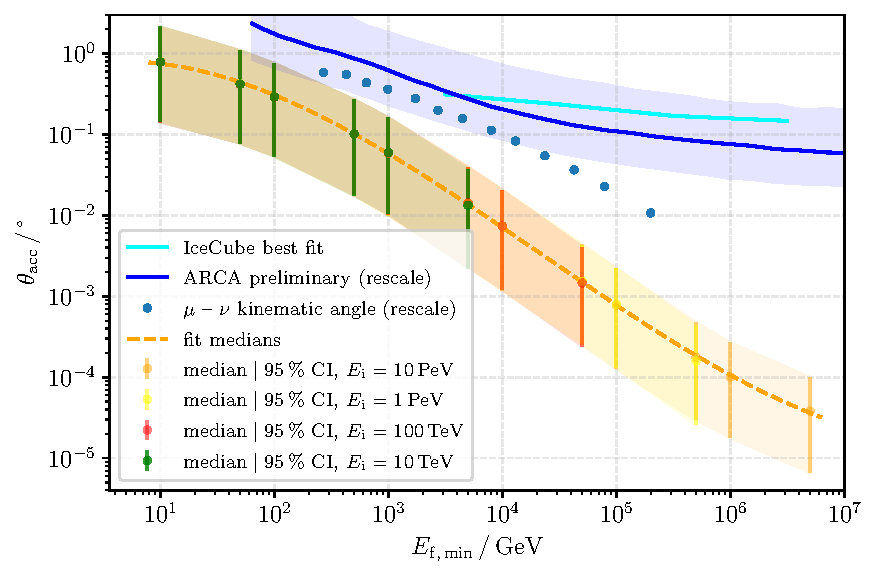
\includegraphics[width=0.96\textwidth]{../../deflection/plots/FINAL/fit_median_defl_cut_10percent_only_poly_new_resolution_rescale_no_icecube_paper_final.pdf}
    \caption{The median of the accumulated deflection $\theta_{\text{acc}}$ in degree 
    with a $\SI{95}{\percent}$ 
    central interval is shown for four different initial energies $E_{\text{i}}$. 
    Each data set includes more than $\num{50000}$ events with the requirement 
    that the true final particle energy $E_{\text{f}}$ is maximum 
    $\SI{10}{\percent}$ below the set final energy $E_{\text{f,\,min}}$,   
    $E_{\text{f}} > E_{\text{f,\,min}} \cdot 0.9$. The energy cuts are $\texttt{e\_cut} = \SI{500}{\mega\electronvolt}$ and $\texttt{v\_cut} = 0.05$ and 
    Molière scattering is chosen. Simulations are done in ice, the deviation 
    of the medians in a water based simulation are less than $\SI{1}{\percent}$.
    Since the medians overlap for different initial energies, there is no 
    strong impact of the initial energy on the median deflection. These 
    medians can be fit by a third degree polynomial in the log-space as 
    shown in Equation~\ref{eqn:fit_median}. For energies 
    $E_{\text{f}} \approx \SI{500}{\giga\electronvolt} - \SI{1}{\tera\electronvolt}$, there is a minimal influence of deflection on the angular resolution of 
    KM3NeT \cite{KM3NeT_Resolution2016}. The resolution of IceCube is not 
    impacted \cite{IceCube_Resolution2021}.}
    \label{fig:fit_median}
\end{figure}

\textcolor{red}{$E_{\text{f}}$ und $E_{\text{f,\,min}}$ eindeutig und konsistent verwenden!}

\textcolor{red}{Fig3 beinhaltet noch keine neutrino-energy korrektur! der neueste plot ist in figures/fit\_median\_defl\_cut\_10percent\_only\_poly\_resolution\_rescale\_no\_icecube.pdf}

% \textcolor{red}{umrechnung der neutrinoenergie in myonenergie: northerntrack sample verwenden, dort einfach reinschauen mit welchen energien werden die neutrinos injeziert, welche muon energien kommen dabei raus -- dieses sample wird verwendet, da es für point source analysis relevant ist -- die gewichtung des spektrums muss berücksichtigt werden -- dort nachschauen, welches spektrum verwendet wird für astro}
